\documentclass[11p]{article}
% Packages
\usepackage{amsmath}
\usepackage{graphicx}
\usepackage[swedish]{babel}
\usepackage[
    backend=biber,
    style=authoryear-ibid,
    sorting=ynt
]{biblatex}
\usepackage[utf8]{inputenc}
\usepackage[T1]{fontenc}
%Källor
\addbibresource{main.bib}
\graphicspath{ {./images/} }

\title{PMmall \\ \small Fysik 1}
\author{Malte Lindkvist}
\date{\today}

\begin{document}

    \begin{titlepage}
        \begin{center}
            \vspace*{1cm}

            \Huge
            \textbf{Vindkraft}

            \vspace{0.5cm}
            \LARGE
            Vindkraftverk

            \vspace{1.5cm}

            \textbf{Malte Lindkvist}

            \vfill

            Ett PM om energiförsörjning \\
            Fysik 1

            \vspace{0.8cm}

            
\includegraphics[width=0.4\textwidth]{NTI Gymnasiet_Symbol_print_svart.png}

            \Large
            Teknikprogrammet\\
            NTI Gymnasiet\\
            Umeå\\
            \today

        \end{center}
    \end{titlepage}
% Om arbetet är långt har det en innehållsförteckning, annars kan den utelämnas

    \newpage
    \section{Inledning}
    El är någonting vi alla använder och kommer använda under de största delar av våra liv, detta betyder att mycket el kommer gå åt, det innebär att vi behöver förnybar energi.
    Det finns flera olika slags förnybar energi, några av dom är vattenkraft, vindkraft och solenergi. Det kallas för en förnybar energikälla eftersom att det ständigt fylls på, t.ex solenergin, solen kommer inte "ta slut" för att vi använder solpaneler medans olja tar slut ifall vi försummar den. Det är alltså energikällor som ständigt fylls på. \parencite{naturskyddsföreningen}

    \section{frågeställningar}
    \begin{enumerate}
        \item Hur fungerar vindkraftverk?
        \item Hur påverkar vindkraftverk miljön?
        \item Hur påverkar vindkraftverk samhället?
    \end{enumerate}


    \section{Vindkraft, så fungerar det}
    Ett vindkraftverk genererar energi genom vinden,
    ett vindkraftverk har en rotor (bladen som snurrar) som driver en generator som sedan producerar el vilket överförs till elnätet. \parencite{Wikipediavindkraftverk}

    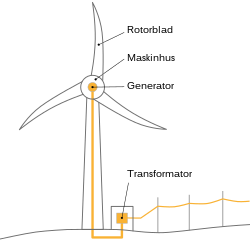
\includegraphics[width=0.4\textwidth]{Vindkraftverk,_principskiss.svg}


    \section{Vindkraft, miljöpåverkan}
    Vindkraft i sig påverkar inte miljön på ett negativt sätt, detta kan dock inte sägas om vindkraftverken.
    Idag är det vanligt att ett vindkraftverk har en rotordiameter på 80-120m och en höjd på 90-100m.\parencite{vindkraftsnyheter}
    Resurserna som gått åt till vindkraftverk är runt 5 miljoner ton stål/järn, 300 000 ton glasfibermaterial, 140 000 ton plaster,
    50 000 ton aluminium och 28 000 ton koppar samt 28 000 ton elektronik till vindkraftverk, kablar och annan elinfrastruktur som behövs för vindkraftsparkerna. \parencite{energimyndigheten}
    Detta betyder att mycket resurser går åt och mycket pengar går också åt, det innebär att vissa delar av naturen blivit konsumerade.
    Vindkraftverken kan påverka Däggdjur och fåglar, för däggdjuren dock är för det mesta bara av uppföringen av vindkraften. Det är då människorna kan skrämma djuren.
    Men fåglarna blir lite mer påverkade, inte nog med att 5-6 fåglar dör tack vare varje vindkraftverk varje år, de blir även störda under uppföringen av vindrkraftverken.\parencite{naturvårdsverket}

    \section{Vindkraftverk, samhällspåverkan}
    Enligt en studie av KTH drar vindkraftverken ner prisen på fastigheterna i en 2km radie runt vindkraftverken.
    Resultatet visade att fastigheterna inom 2km av ett vindkraftverk var i genomsnitt 13.2 procent lägre än de som var längre ifrån vindkraftverken under åren 2012-2018 och
    10.9 procent lägre under 2005-2011 på grund av närhet till vindkraft.\parencite{motvindsverige}

    \section{Slutsatser}
Det finns fördelar och nackdelar med vindkraft, men jag har kommit fram till att fördelarna utväger nackdelarna eftersom att ett vindkraftverk kan årliga producera tillräckligt mycket el för 4000 hushåll.\parencite{vattenfall}



    \printbibliography

\end{document}
